\documentclass[magyar]{beamer}
\usepackage[T1]{fontenc}
\usepackage[utf8]{inputenc}
\usepackage{verbatim}
\usepackage{beamerthemeboxes}
\PassOptionsToPackage{normalem}{ulem}
\usepackage{ulem}
\usepackage{moreverb}
\usetheme{Madrid}
\usepackage{tikz} 
\usetikzlibrary{shapes}
\makeatother

\usepackage{babel}

\defbeamertemplate*{footline}{mytheme}
{
  \leavevmode%
  \hbox{%
  \begin{beamercolorbox}[wd=.5\paperwidth,ht=2.25ex,dp=1ex,center]{author in head/foot}%
	    \usebeamerfont{author in head/foot}{Nagy Zoltán Arnold}~~
  \end{beamercolorbox}%
  \begin{beamercolorbox}[wd=.5\paperwidth,ht=2.25ex,dp=1ex,right]{date in head/foot}%
    \usebeamerfont{date in head/foot}{AsiaBSDCon 2012, Tokyo, Japan}\hspace*{2em}
    \insertframenumber{} / \inserttotalframenumber\hspace*{2ex}
  \end{beamercolorbox}}%
  \vskip0pt%
}
\usebeamertemplate{mytheme}
\beamertemplatenavigationsymbolsempty
\date{}
\begin{document}

\title{NPF: a new packet filter}
\author{Zoltán Arnold Nagy \\ The NetBSD Foundation \\ zoltan@netbsd.org}
\maketitle

\begin{frame}
\begin{itemize}
	\item What is a packet filter?
\pause
	\begin{itemize}
		\item A boolean valued function ($f:\mathbb{P} \rightarrow \mathbb{B}$)
	\end{itemize}
\pause
	\item How can it be implemented?
\pause
	\begin{itemize}
		\item boolean expression tree
		\item directed acyclic control flow graph\footnote{The graph on the next page is taken from "The BSD Packet Filter: A New
Architecture for User-level Packet Capture" by Steven McCanne and Van Jacobson}
		\item if-then-else hell
	\end{itemize}
\end{itemize}
\end{frame}

\begin{frame}
\begin{center}
	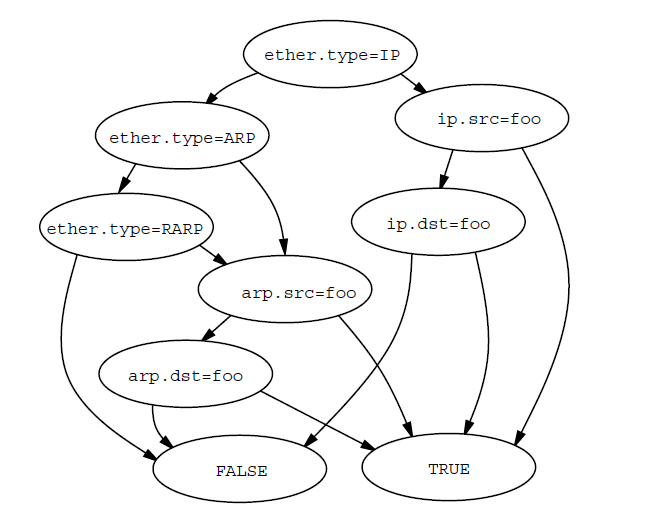
\includegraphics[scale=.5]{cfg}
\end{center}
\end{frame}

\begin{frame}
\frametitle{A sea of firewalls}
\begin{itemize}
	\item IPFilter (ipf)
	\item FreeBSD's ipfw
	\item OpenBSD's pf
	\item NetBSD's npf
\end{itemize}
\end{frame}

\begin{frame}
\frametitle{How NPF started out}
\begin{itemize}
	\item Sponsored by The NetBSD Foundation
	\item Written by Mindaugas Rasiukevicius (rmind@) from scratch, altought the design was inspired by the Berkeley Packet Filter
	\item First imported to -current in August 2010
\end{itemize}
\end{frame}

\begin{frame}
\frametitle{Google Summer of Code}
\begin{itemize}
	\item Goal: The program's goal is to promote open-source software development among students and get them actually involved
\pause
	\item Mentoring organizations apply with a set of proposed projects
\pause
	\item Students apply for organizations with a proposal based either on a proposed project or a new one
\pause
	\item Organizations get a number of slots for students
\pause
	\item Mentoring organizations get \textdollar500 per student, students get \textdollar5000
\pause
	\item It has been running since 2005
		\begin{itemize}
			\item 2011: 175 mentoring organizations, 1115 students
		\end{itemize}
	\item NetBSD has participated every year so far with a high success rate
		\begin{itemize}
			\item 2011: 9 projects, 8 projects ended with success
			\item Already accepted for 2012 as a mentoring organization
		\end{itemize}
	\item My GSoC proposal for 2011 was to add IPv6 support to NPF
		\begin{itemize}
			\item committed to -current in November 2011
		\end{itemize}
	\item Something will happen in 2012 too :-)
\end{itemize}
\end{frame}

\begin{frame}
\frametitle{Motivations and goals}
\begin{itemize}
	\item There are a few existing firewalls
	\item It's easier to design a new firewall from ground up than to clean up existing codebases
	\item Design goals for NPF:
	\begin{itemize}
		\item MP-safety and locklessness for scalable MP performance
		\item Fast tree- and hash-based lookup support for tables
		\item Stateful packet filtering
		\item N-Code processor, a general bytecode engine
		\item Keep configuration syntax changes to a minimum
		\item Modularity, extensibility: an extension API for developers, hooking support
		\item Last but not least: simplicity
	\end{itemize}
	\item Of course it's portable, uses pfil(9) hooks; DragonFlyBSD is considering adoption 
	\item Work in progress
\end{itemize}
\end{frame}

\begin{frame}
\frametitle{Usage}
\begin{itemize}
	\item \texttt{npfctl} can be used to communicate with /dev/npf via ioctls
		\begin{itemize}
			\item start, stop, reload, flush, stats, tables, sessions, ...
		\end{itemize}
	\item Rules are translated into bytecode, and pushed down to the kernel
	\item The parser has been recently rewritten by christos@ based on martin@'s code
\end{itemize}
\end{frame}

\begin{frame}[fragile]
\frametitle{Features - variables and groups}
\begin{itemize}
	\item Each group has a name and an interface defined
	\item If there's no deciding rule in the custom group, the default group's rules will be inspected
	\item It's important to mark any deciding rule final ("quick")
\end{itemize}
\begin{verbatim}
ext_if = "wm0"
int_if = "wm1"

group (name "external", interface $ext_if) {
    ...
}

group (name "internal", interface $int_if) {
    ...
}

group (default) {
    block all
}
\end{verbatim}
\end{frame}

\begin{frame}[fragile]
\frametitle{Features - rule procedures}
\begin{itemize}
	\item Allows connection-based packet transformation
	\item If made pluggable, would allow kernel modules to perform custom packet modifications
	\item Currently 
\end{itemize}
\begin{verbatim}
procedure "rid" {
    normalize (random-id)
}

procedure "log" {
    log npflog0
}
\end{verbatim}
\end{frame}

\begin{frame}[fragile]
\frametitle{Features - tables}
\begin{verbatim}
table "1" type tree dynamic
table "2" type hash file "/etc/npf_backlist"

group (default) {
    block in quick from <1>
    block out quick to <2>
}
\end{verbatim}
\end{frame}

\begin{frame}
\frametitle{Features - Application Level Gateways}
\begin{itemize}
	\item Some protocols embed lower level information in their payload (think FTP's PORT, SIP, RTSP)
	\item In order to dynamically handle these, we need to actually process the data
	\item This is mostly important for NAT setups
	\item Currently there's only one ALG implemented for ICMP (traceroute support)...
\end{itemize}
\end{frame}

\begin{frame}
\frametitle{What can it do today?}
\begin{itemize}
	\item Rule syntax is nearly identical to other firewalls
	\item Group support
	\item Rule procedures (connection-based packet transformations)
	\begin{itemize}
		\item IP ID randomization
		\item enforcement of TCP minimum TTL
		\item enforcement of TCP Maximum Segment Size (MSS)
		\item logging
	\end{itemize}
	\item Tables support
	\item Application-level gateways (ALGs)
\end{itemize}
\end{frame}

\begin{frame}[fragile,basicstyle=\ttfamily]
\begin{verbatim}
ext_if = "wm0"
int_if = "wm1"
table "1" type "tree" dynamic
procedure "rid" { normalize (random-id) }
procedure "log" { log npflog0 }
group (name "external", interface $ext_if) {
    block in quick from <1>
    pass out quick from $ext_if keep state apply "rid"
    pass in quick proto tcp to $ext_if port ssh apply "log"
    ...
}
group (name "internal", interface $int_if) {
    block in all
    pass in quick from <1>
    pass out quick all
}
group (default) { block all }
\end{verbatim}
\end{frame}

\begin{frame}
\frametitle{Inside}
N-code engine:
\begin{itemize}
	\item General purpose bytecode engine, 32-bit words, 4 registers available
	\item The firewall configuration is compiled to our bytecode format, then loaded
	\item CISC and RISC-like instructions
	\item The packets are processed as a byte-stream
\end{itemize}
Efficient internal structures
\begin{itemize}
	\item npf\_addr (in6\_addr, 128-bit) for addresses (the first 32 bit is used for IPv4 addresses)
	\item uint8\_t for masks
	\begin{itemize}
		\item instead of generating the appropriate npf\_addr value from the netmask(255.255.255.0 or /24), we just store
the mask
		\item tradeoff: CPU for memory
	\end{itemize}
\end{itemize}
\end{frame}

\begin{frame}[fragile]
\frametitle{Inside}
Let's see what we can work with...
{\tiny
\begin{verbatim}
typedef struct {
        /* Information flags. */
        uint32_t                npc_info;
        /* Pointers to the IP v4/v6 addresses. */
        npf_addr_t *            npc_srcip;
        npf_addr_t *            npc_dstip;
        /* Size (v4 or v6) of IP addresses. */
        int                     npc_ipsz;
        size_t                  npc_hlen;
        int                     npc_next_proto;
        /* IPv4, IPv6. */
        union {
                struct ip       v4;
                struct ip6_hdr  v6;
        } npc_ip;
        /* TCP, UDP, ICMP. */
        union {
                struct tcphdr   tcp;
                struct udphdr   udp;
                struct icmp     icmp;
        } npc_l4;
} npf_cache_t;
\end{verbatim}
}
\end{frame}

\begin{frame}
\frametitle{TODOs after the 6.0 release}
\begin{itemize}
	\item Replace red-black trees with (lockless) Patricia (radix) trees for tables
\pause
	\item Pregenerate an array for masks, and allow run-time switching
\pause
	\item Support per-rule statistics
\pause
	\item Multiple address per interface support on interface-based rules
	\item Dynamic interface tracking
		\begin{itemize}
			\item Let's say you have a rule based on an interface instead of an address...
			\item ...you compile and load the rules...
			\item ...then change the interface's address?
		\end{itemize}
	\item Control fragmentation on a per-interface basis
\pause
	\item Stateful NAT64 [RFC 6146]
	\item IPv6-to-IPv6 Network Prefix Translation (NPTv6) [RFC 6296]
\pause
	\item Port over to FreeBSD in order to prove our performance claims :-)
\pause
	\item Write more documentation and fix remaining bugs
\end{itemize}
\end{frame}

\begin{frame}
\frametitle{Additional ideas}
\begin{itemize}
	\item Spread the RX/TX queue processing on modern NICs across all cores
\pause
	\item Optimize the ruleset
	\begin{itemize}
		\item first step could be to prune the graph based on heuristics
		\item then to compile it to actual machine code (JIT/LLVM/...)
	\end{itemize}
\pause
	\item Make the network stack lockless, but this is a daunting task
\end{itemize}
\end{frame}

\begin{frame}
\begin{center}
Questions and answers?
\end{center}
\end{frame}

\begin{frame}
\begin{center}
Arigatou gozaimashita!
\end{center}
\end{frame}

\end{document}
